\documentclass{article}

\usepackage{float,algorithm,graphicx,hyperref,amsmath,amsfonts,verbatim}
\usepackage[noend]{algpseudocode}

\title{Lab 4 - Non-Linear Classifiers and Kernels}
\author{Kyle Swanson}
\date{January 15, 2018}

\setcounter{section}{-2}

\begin{document}

\maketitle

\section{Installation}

Before you begin the lab, you will need to install a Python tool called \texttt{tqdm}, which displays progress bars. It's useful since some of the methods we write will run a little slowly and we will want to know how close they are to finishing. To install it, run the following in your terminal:

\vspace{2mm}

\begin{center}
    \texttt{pip install tqdm}
\end{center}

\section{Introduction}

Up until this point, we've been working solely with linear classifiers because they are easy to understand and implement. However, most data sets you will encounter in the real world cannot be separated by a simple linear classifier $-$ usually the underlying distribution of the data is much more complicated.

The goal of this lab is to develop your skills working with non-linear classifiers since these classifiers can classify a much broader range of data sets. We will do so using two related methods: data transformations and kernels.

\subsection{Data transformations}

Data transformation involves taking a data set which is not linearly separable and computing a function, $\phi$, which transforms the data set into a new data set which is linearly separable. Specifically, if our training set is

$$S_n = \left\{\left(x^{(1)}, y^{(1)}\right),\ \left(x^{(2)}, y^{(2)}\right),\ \dots,\ \left(x^{(n)}, y^{(n)}\right)\right\}$$

\noindent
then our goal is to find a function $\phi$ such that if we transform each data point $x^{(i)}$ with $\phi$, then the transformed data set

$$S'_n = \left\{\left(\phi(x^{(1)}),\ y^{(1)}\right),\ \left(\phi(x^{(2)}), y^{(2)}\right),\ \dots,\ \left(\phi(x^{(n)}), y^{(n)}\right)\right\}$$

\noindent
is linearly separable. The choice of $\phi$ will depend entirely on the data under consideration. Once $\phi$ is chosen, we will train a linear classifier on the transformed data set $S'_n$, which will be equivalent to training a non-linear classifier on the original data set $S_n$.

\subsection{Kernels}

The kernel method implicitly involves the same data transformation process, but it uses kernel functions to avoid explicitly computing the data transformation function $\phi$. Using kernel methods, we will continue to use the original data set $S_n$, but our linear classifier will be modified to use the kernel function when computing the linear classifier $\theta$ in order to simulate the data transformation process.

Although the kernel method is a little more complicated than the data transformation method, it avoids computing the data transformation function $\phi$, which can make it significantly more efficient when complex data transformations are required.

\section{Kernel Perceptron}

Your first task is to implement the kernel perceptron algorithm, which is a non-linear version of the perceptron algorithm:

\begin{algorithm}[H]
    \caption{Kernel Perceptron Algorithm}
    \label{perceptron}
    
    \begin{algorithmic}[1]
        \Procedure{Kernel Perceptron}{}
        \State $\alpha^{(1)}, \alpha^{(2)}, \dots, \alpha^{(n)} = 0$
        \For{$t = 1, 2, \dots, T$}
            \For{$i = 1, 2, \dots, n$}
                \If{$\textrm{sign} \left(\sum_{j=1}^n \left(\alpha^{(j)} y^{(j)} k \left( x^{(j)}, x^{(i)} \right) \right) \right) \neq y^{(i)}$}
                    \State $\alpha^{(i)} = \alpha^{(i)} + 1$
                \EndIf
            \EndFor
        \EndFor
        \EndProcedure
    \end{algorithmic}
\end{algorithm}

In \texttt{lab4.py} you will find a class called \texttt{KernelPerceptron} with two functions, \texttt{fit} and \texttt{predict}. This should look familiar to the methods used by scikit-learn models $-$ in fact, our KernelPerceptron is actually going to be implemented as a custom scikit-learn model.

First you will implement \texttt{fit}. This function takes in a set of data points \texttt{X} and a set of labels \texttt{y} and learns a vector of $\alpha$ values called \texttt{self.alpha}. The $i^{th}$ element of \texttt{self.alpha} should contain the number of mistakes made by the perceptron on the $i^{th}$ data point.

Next you will implement \texttt{predict}. This function takes in a set of data points \texttt{X} and returns an array of predictions for each data point. You will need to use the values of \texttt{self.alpha} learned in the \texttt{fit} method to make these predictions. Remember, the predicted label for data point $x^{(i)}$ is

$$\textrm{sign} \left( \sum_{j=1}^n \left( \alpha^{(j)} y^{(j)} k \left( x^{(j)}, x^{(i)} \right) \right) \right)$$

Once your implementation is complete, proceed to part \ref{linear} where your implementation will be tested.

\begin{comment}

\subsection{How it works}

Remember that our goal is to use kernel functions to simulate the data transformation function $\phi$ without actually computing it.

Remember that $\alpha^{(i)}$ represents the number of mistakes that the perceptron makes on example $x^{(i)}$. Since we add $y^{(i)} x^{(i)}$ to $\theta$ every time we make a mistake on example $x^{(i)}$, you'll see that we can rewrite $\theta$ as follows:

$$\theta = \alpha^{(1)} y^{(1)} x^{(1)} + \alpha^{(2)} y^{(2)} x^{(2)} + \dots + \alpha^{(n)} y^{(n)} x^{(n)} = \sum_{i=1}^n \alpha^{(i)} y^{(i)} x^{(i)}$$

Now instead of computing

$$y^{(i)} \left( \theta \cdot x^{(i)} \right) \leq 0$$

\noindent
to determine whether there is a mistake, we can compute

$$y^{(i)} \left(\left(\alpha^{(1)} y^{(1)} \phi(x^{(1)}) + \alpha^{(2)} y^{(2)} \phi(x^{(2)}) + \dots + \alpha^{(n)} y^{(n)} \phi(x^{(n)})\right) \cdot \phi(x^{(i)}) \right)$$

\subsection{How it works}

(Note: The following is not necessary for completing the lab, but it helps explain some of the math that makes the kernel perceptron work.)

Remember that the kernel perceptron doesn't directly compute $\theta$ but instead computes $\alpha^{(i)}$'s, which represent the number of mistakes made on training example $x^{(i)}$. Additionally, instead of computing the regular dot product between $x^{(i)}$ and $\theta$, the kernel perceptron uses the kernel function $k$ to compute a (potentially) non-linear version of the dot product.

We can see below how this kernel method is equivalent to using regular perceptron with the data transformation method. Remember that in regular perceptron, we check for mistakes by checking whether $y^{(i)} \left( \theta \cdot x^{(i)} \right) \leq 0$. When we use transformed data $\phi(x^{(i)})$, we check whether $y^{(i)} \left( \theta \cdot \phi(x^{(i)}) \right) \leq 0$. Below we start with the data transformation version and derive the kernel version:

$$y^{(i)} \left( \theta \cdot \phi(x^{(i)} \right)$$
$$= y^{(i)} \left(\left(\alpha^{(1)} y^{(1)} \phi(x^{(1)}) + \alpha^{(2)} y^{(2)} \phi(x^{(2)}) + \dots + \alpha^{(n)} y^{(n)} \phi(x^{(n)})\right) \cdot \phi(x^{(i)}) \right)$$
$$= y^{(i)} \left(\alpha^{(1)} y^{(1)} \phi(x^{(1)}) \cdot \phi(x^{(i)}) + \alpha^{(2)} y^{(2)} \phi(x^{(2)}) \cdot \phi(x^{(i)}) + \dots + \alpha^{(n)} y^{(n)} \phi(x^{(n)}) \cdot \phi(x^{(i)})\right)$$
$$= y^{(i)} \left(\alpha^{(1)} y^{(1)} k(x^{(1)}, x^{(i)}) + \alpha^{(2)} y^{(2)} k(x^{(2)}, x^{(i)}) + \dots + \alpha^{(n)} y^{(n)} k(x^{(n)}, x^{(i)})\right)$$
$$=y^{(i)} \sum_{j=1}^n \left( \alpha^{(j)} y^{(j)} k(x^{(j)}, x^{(i)}) \right)$$

(Note that by definition of the kernel, we have $\phi(x^{(j)}) \cdot \phi(x^{(i)}) = k(x^{(j)}, x^{(i)})$.)

\end{comment}

\section{Linear Models} \label{linear}

Now we will begin using your implementation of the Kernel Perceptron algorithm, along with scikit-learn's implementation of the SVM algorithm, to learn various linear and non-linear classifiers.

First, run \texttt{main.py} without modifying it. You'll see the following four graphs pop up:

\noindent
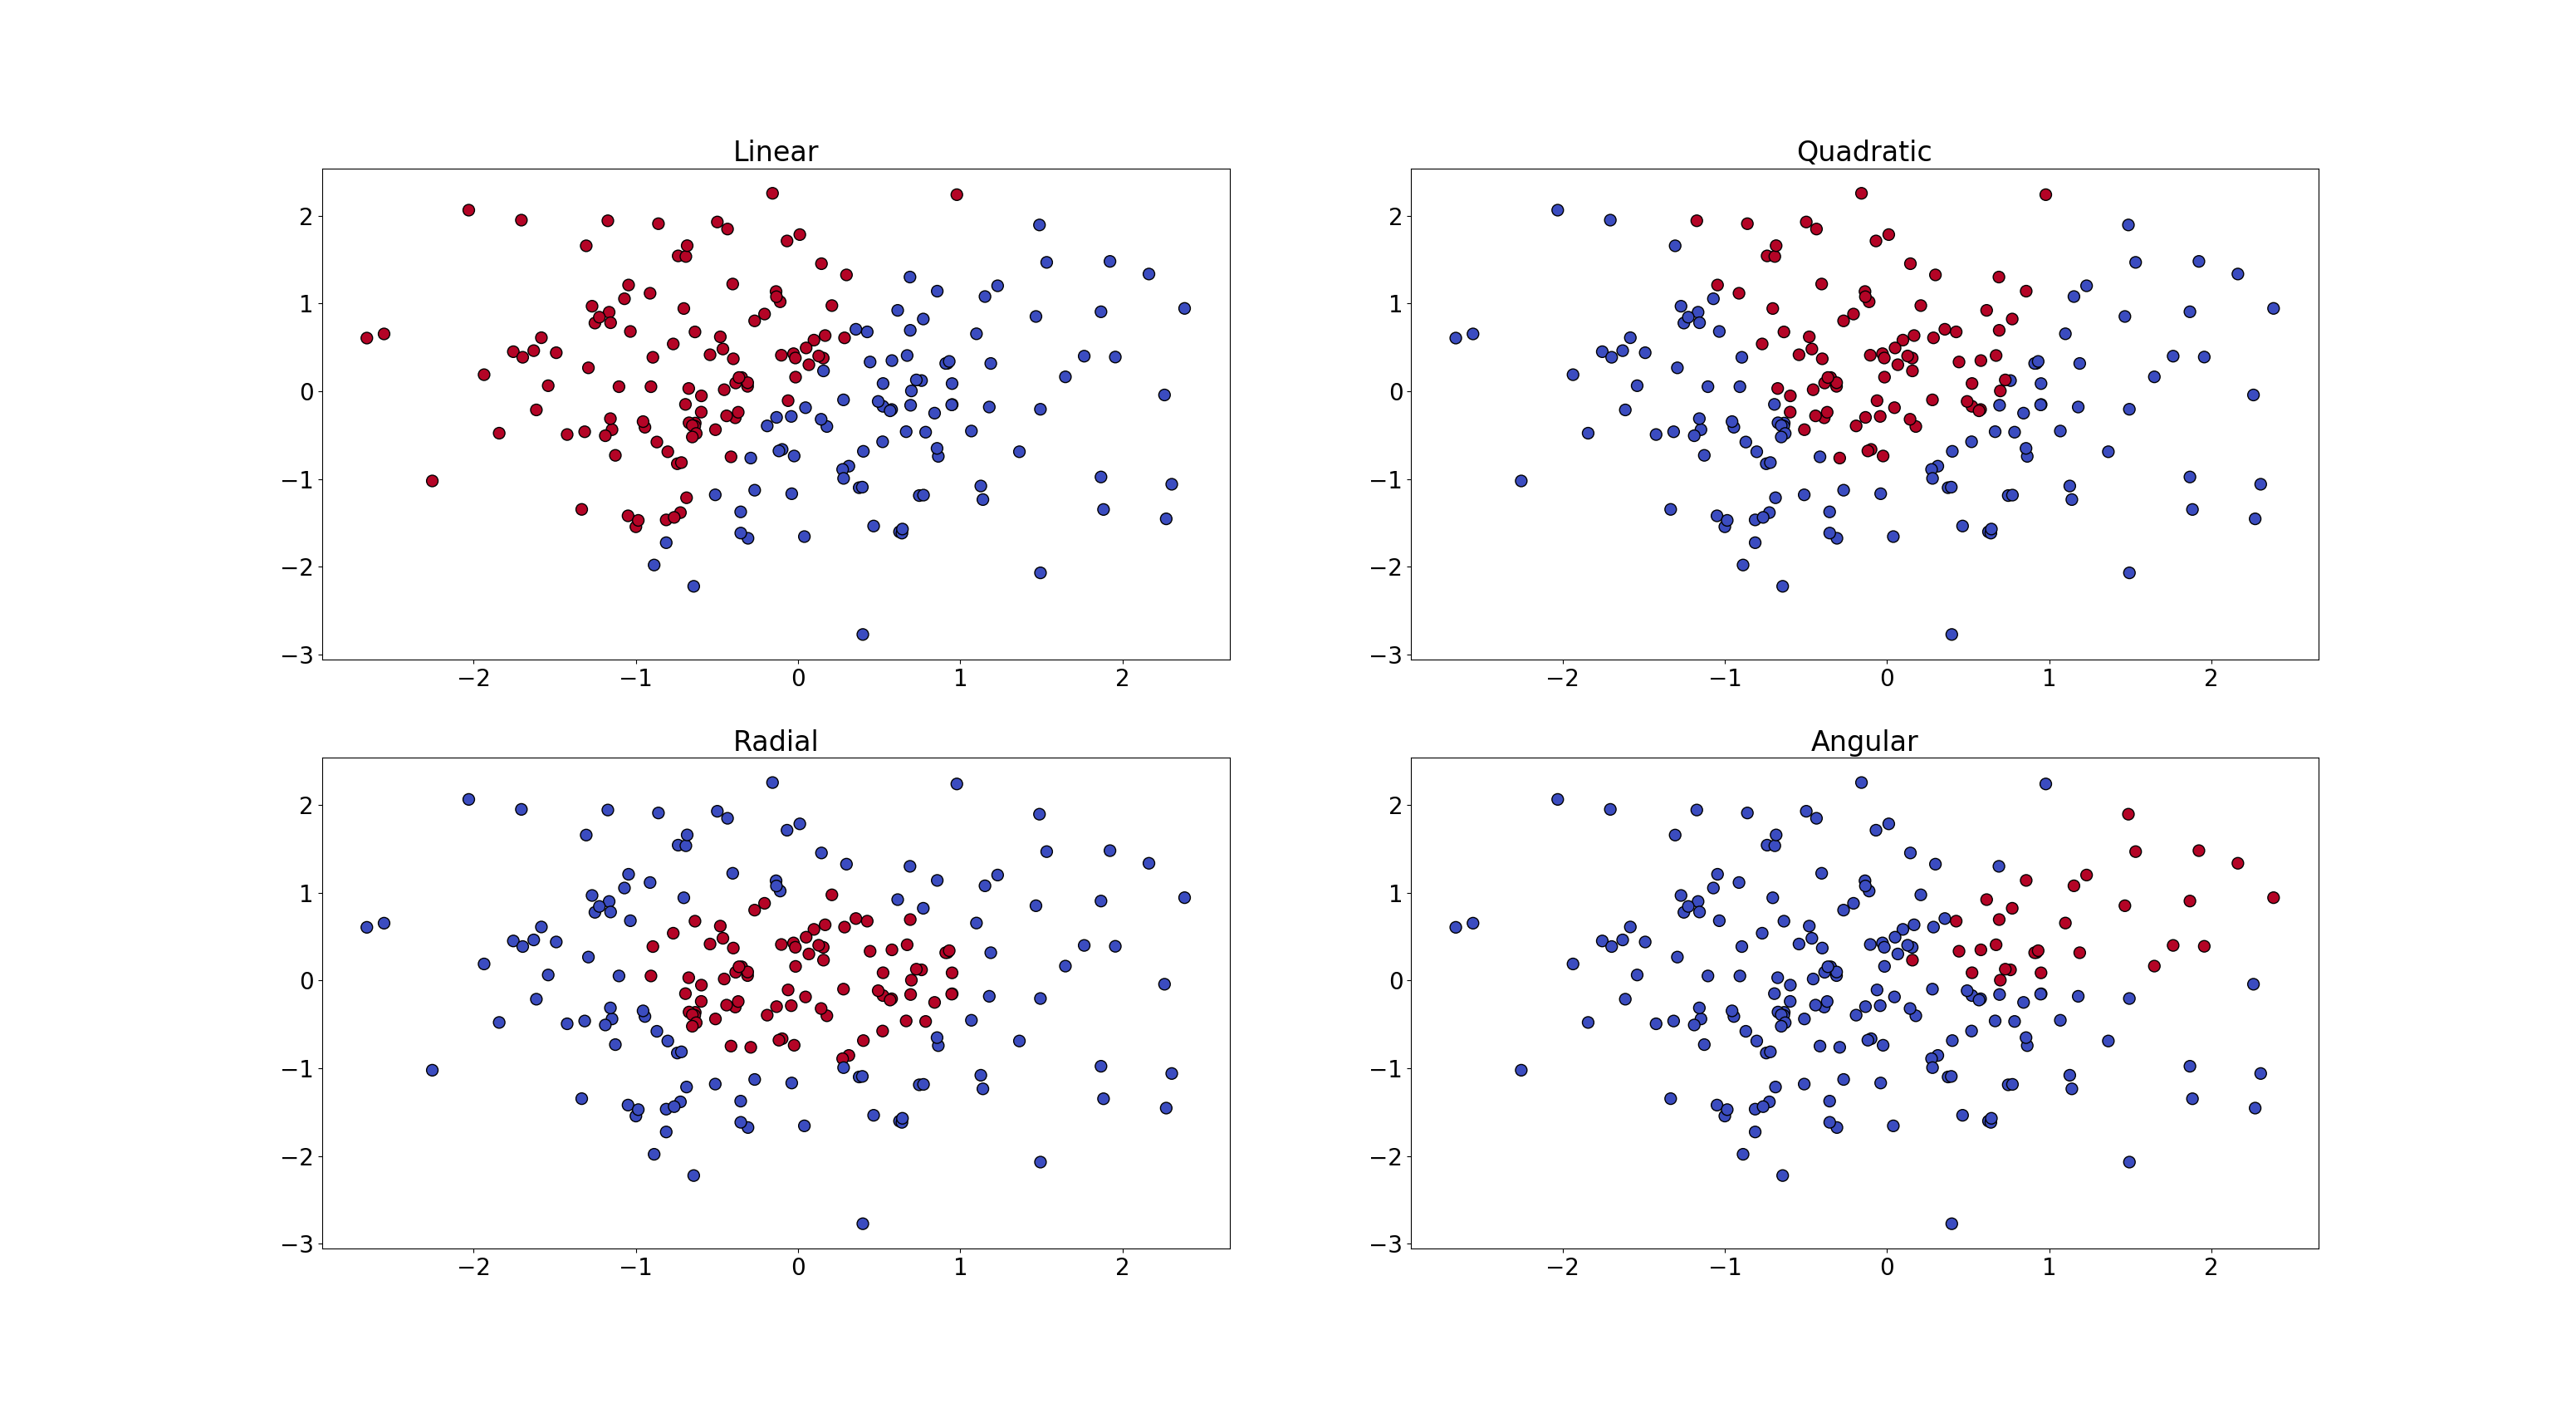
\includegraphics[width=\textwidth]{datasets.png}

These are the four data sets that we will try to classify in this lab.

\vspace{2mm}

We will begin by tackling the first data set, which is linearly separable.

\noindent
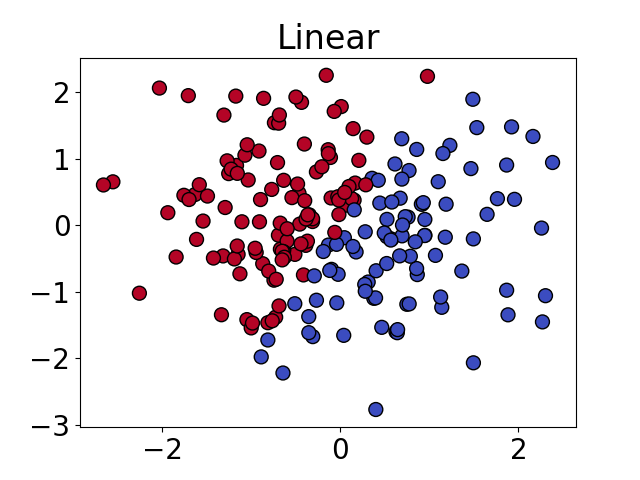
\includegraphics[width=\textwidth]{linear.png}

Uncomment Part 2 in \texttt{main.py}. Since the data is linearly separable, we need to give the KernelPerceptron a linear kernel. A linear kernel is simply the regular dot product:

$$k \left( x^{(j)}, x^{(i)} \right) = x^{(j)}\cdot x^{(i)}$$

(Note: If you study the algorithm carefully, you'll see that KernelPerceptron with a linear kernel is actually identical to the regular perceptron algorithm, which we already know is capable of learning a linear classifier.)

Implement the function \texttt{linear\_kernel} using the above definition of $k \left( x^{(j)}, x^{(i)} \right)$ and then run \texttt{main.py}. You should see two graphs pop up, both with similar linear classifiers. The one on the left is the classifier learned by your KernelPerceptron algorithm while the one on the right is the classifier learned by scikit-learn's linear SVM model. If the two graphs look different, let me know and I can check your KernelPerceptron to make sure it's correct.

\section{Quadratic Models}

Now we can finally tackle our first non-linear data set. We will begin with the following data set, which is only separable with a quadratic classifier:

\noindent
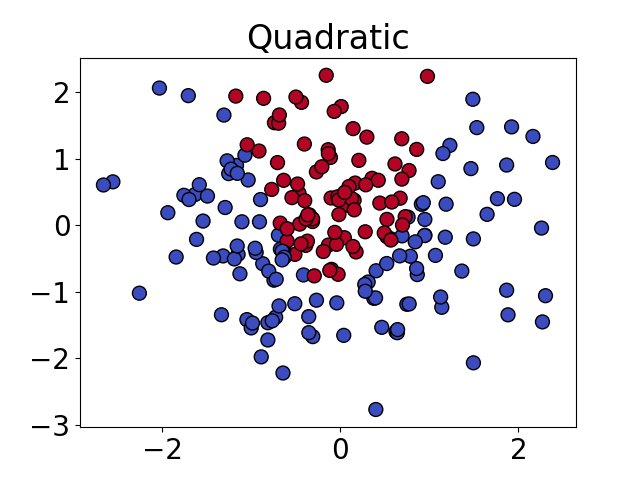
\includegraphics[width=\textwidth]{quadratic.png}

We will build a classifier in two ways, first with a data transformation, then with a kernel.

\subsection{Quadratic Data Transformation}

In order to build a quadratic classifier by using a linear classifier on transformed data, we need to choose a function $\phi$ which can transform our data set into a data set which is linearly separable.

Uncomment Part 3.1 in \texttt{main.py}. Your job is to implement the function \texttt{phi\_quad}, which takes in a vector \texttt{x} and returns a transformed vector $\phi(x)$ such that the transformed data is now linearly separable (see below for a hint).

When you're done, run \texttt{main.py}. You should see three graphs: one with the original data, one with a linear classifier trained on your transformed data, and one with a projection of your linear classifier back onto the original data set. You can see that by learning a linear classifier on the transformed data data, we get a non-linear classifier on the original data.

\subsubsection{Hint}

Choosing the right function $\phi$ will take a bit of thinking. Think about the relationship between the $x_1$ and $x_2$ dimensions of each data point. Since the relationship is quadratic, we know that the data point is red if $a * x_1^2 + b > x_2$ (for some real numbers $a$ and $b$) and the data point is blue if $a * x_1^2 + b \leq x_2$. So how could we transform $x =
\begin{bmatrix}
    x_1 \\
    x_2
\end{bmatrix}$ into a new vector so that the relationship between $x_1$ and $x_2$ is linear instead of quadratic? If you're not sure, come talk to me and we can work through it together.

\subsection{Quadratic Kernel}

In this section, we will build a quadratic classifier by using a quadratic kernel instead of a quadratic data transformation. Coming up with a quadratic kernel on your own is not easy, so here is the quadratic kernel:

$$k \left( x^{(j)}, x^{(i)} \right) = \left( x^{(j)} \cdot x^{(i)} \right)^2 + 2 * \left( x^{(j)} \cdot x^{(i)} \right) + 1$$

Uncomment Part 3.2 in \texttt{main.py} and implement the function \texttt{quad\_kernel} with the above kernel. Now run \texttt{main.py}. You should see a single graph showing the non-linear classifier learned by your KernelPerceptron algorithm with the quadratic kernel.

\section{Radial Models}

Next we will examine another non-linear data set:

\noindent
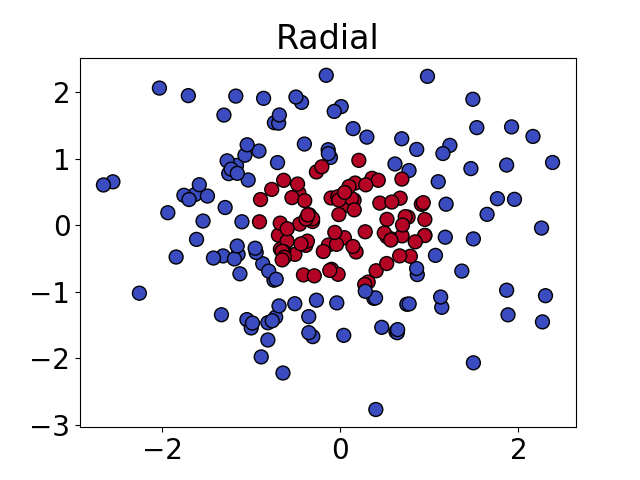
\includegraphics[width=\textwidth]{radial.png}

As with the quadratic models, we will implement a radial classifier both with the data transformation method and with the kernel method.

\subsection{Radial Data Transformation}

Uncomment Part 4.1 in \texttt{main.py}. Your job is to implement \texttt{phi\_radial}, which needs to transform the data points into linearly separable data points. Let me know if you're having trouble coming up with the right function.

Once you've implemented the function, run \texttt{main.py}. As with the quadratic data transformation, you should see three graphs: one with the original data, one with a linear classifier trained on your transformed data, and one with a projection of your linear classifier back onto the original data set.

\subsection{Radial Kernel}

Uncomment Part 4.2 in \texttt{main.py}. Here you need to implement the function \texttt{radial\_kernel}. This function computes the radial basis kernel, which is as follows:

$$k \left( x^{(j)}, x^{(i)} \right) = \exp \left( {\frac{||x^{(j)} - x^{(i)}||^2}{2}} \right)$$

Once your implementation is complete, run \texttt{main.py}. You should see two graphs. The one on the left displays the non-linear classifier learned by your KernelPerceptron algorithm with the radial basis kernel you just implemented, while the graph on the right shows scikit-learn's radial SVM model on the same data.

\section{Angle Models}

Here's one last data set for which we will build a non-linear classifier:

\noindent
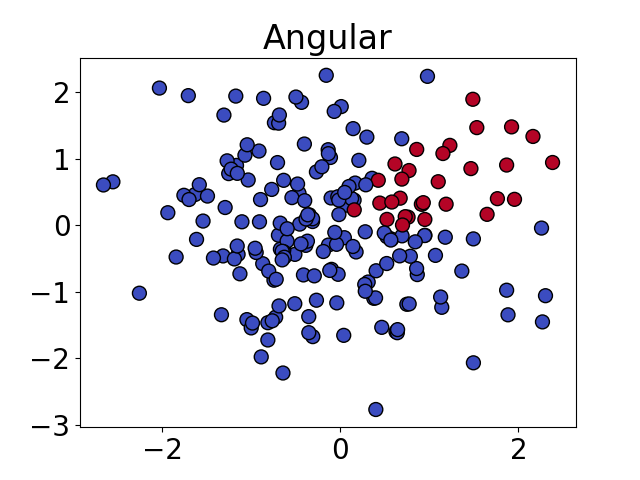
\includegraphics[width=\textwidth]{angular.png}

Note that the label of the data points (red or blue) depends on the angle of the data point (the origin is at the center of the graph above), meaning we're going to need a data transformation which allows us to build an angle-based classifier.

\vspace{2mm}

Uncomment the code in Part 5. This time we are only going to do a data transformation and not a kernel. Your job is to implement \texttt{phi\_angular}, which transforms data points so that the resulting data points are linearly separable. In my opinion, this is a much harder transformation to think of. If you can't figure it out, come talk to me and I'll give you some hints.

Once you have implemented \texttt{phi\_angular}, run \texttt{main.py}. As usual, you should see three graphs: one with the original data, one with a linear classifier trained on your transformed data, and one with a projection of your linear classifier back onto the original data set.

\section{Bonus: k-Nearest Neighbors}

While this isn't directly related to data transformations and kernels, another method of building a non-linear classifier is through the k-nearest neighbors (KNN) algorithm. To predict the label of a new data point $x$, the KNN algorithm works by looking at the $k$ training data points which are nearest to $x$, and it predicts the majority label among those data points. So for example, if $k=3$ and the three training points closest to $x$ have labels red, red, and blue, then the prediction for $x$ would be red since the majority of the $3$ nearby training points are red.

Uncomment the code in Part 6 of \texttt{main.py} and run \texttt{main.py}. You'll see several graphs appear. The first is the original data set (note that there are now 5 possible labels (colors) rather than just 2), and the rest are the predictions of the $k$ nearest neighbors algorithm for different values of $k$. Which value of $k$ do you think works best?

\end{document}
